%\documentclass[margin=0pt]{standalone}
%\usepackage{tikz}
\usetikzlibrary{3d}

\begin{document}

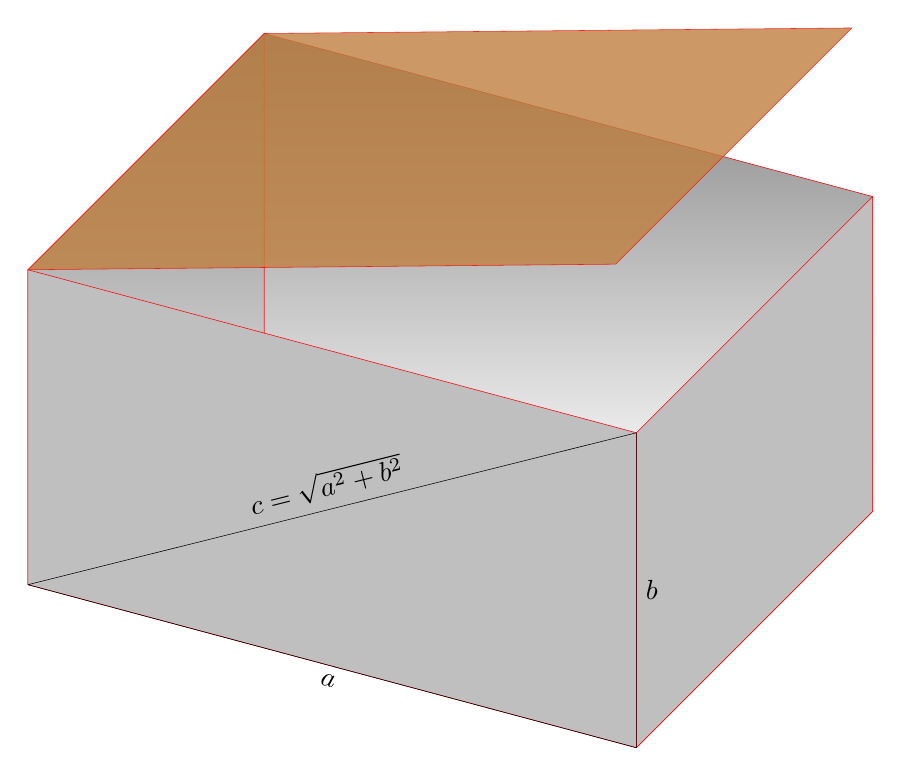
\begin{tikzpicture}[
        x = {(-0.5cm,-0.5cm)},
        y = {(0.9659cm,-0.25882cm)},
        z = {(0cm,1cm)},
        scale = 2,
        color = {lightgray}
    ]
    % style of faces
    \tikzset{facestyle/.style={fill=lightgray,draw=red,very thin,line join=round}}
    % face "back" 
    \begin{scope}[canvas is zy plane at x=0]
        \path[facestyle,shade] (0,0) rectangle (2,4);
    \end{scope}
    % face  "left"
    \begin{scope}[canvas is zx plane at y=0]
        \path[facestyle,shade] (0,0) rectangle (2,3);
    \end{scope}
    % face "front"
    \begin{scope}[canvas is zy plane at x=3]
        \path[facestyle] (0,0) rectangle (2,4);
    \end{scope}
    % face  "right"
    \begin{scope}[canvas is zx plane at y=4]
        \path[facestyle] (0,0) rectangle (2,3);
    \end{scope}
    % face "up" 
    \draw[fill=brown,draw=red,opacity=.8,very thin,line join=round]
    (0,0,2) -- 
    (3,0,2) --
    (3,{4*cos(15)},{4*sin(15)+2}) --
    (0,{4*cos(15)},{4*sin(15)+2}) --cycle ;
    % labels
    \draw[very thin,black,line join=round]
    (3,0,0) -- node [sloped,below] {$a$}    
    (3,4,0) -- node [right]        {$b $}
    (3,4,2) -- node [sloped,above] {$c=\sqrt{a^2+b^2}$} 
    (3,0,0);
\end{tikzpicture}

\end{document}
